\documentclass[../../../main.tex]{subfiles}

\begin{document}

\section{Geometry in 3-Space}

In this section of the note, we will discuss more geometric
analysis in 3-space with vectors. I personally think it was
very interesting to see different interpretations of vectors
in 3-space because they could be very abstract, yet a fundamental
component that helps analyzing geometry in 3-dimensions.

\subsection{Lines in 3-Space}

Continuing with our prior discussion on vectors, let's discuss
more on lines and planes in 3-space and how they relate to vectors.

First, the components of lines in the coordinate plane can be thought
of as a point and a direction, which would be slope. Given a point
that a line passes through and the slope, or direction, of the line,
we can find the unique line. Similarly, we could do the same for
3-space. The direction in this case would be a nonzero vector.
In other words, given a point and a nonzero vector parallel to
the line, we can find the unique line.

\begin{figure}[H]
\centering
\tdplotsetmaincoords{70}{110}
\begin{tikzpicture}[
        tdplot_main_coords,
        axis/.style={->,thick},
        scale=0.4
    ]
    \draw[axis] (-8,0,0) -- (8,0,0) node[left] {$x$};
    \draw[axis] (0,-7,0) -- (0,8,0) node[right] {$y$};
    \draw[axis] (0,0,-5) -- (0,0,8) node[left] {$z$};

    \draw[axis] (0,0,0) -- (-0.5,3,1.5) node[right]
        {$\langle a, b, c \rangle$};
    \draw[Red] (2,-3,3) -- (1,3,6) node[below] {$l$};
    \node[circle,fill=black,inner sep=0pt,minimum size=1mm]
        at (0,0,0) {};
    \node[circle,fill=black,inner sep=0pt,minimum size=1mm]
        at (1.5, 0, 4.5) {};
    \node[above left] at (1.5, 0, 4.5) {$(x_0, y_0, z_0)$};
\end{tikzpicture}
\end{figure}

Looking at the graph above, we can derive a very important
concept of representing lines in parametric equations.

\begin{important}
A line $l$ in 3-space that passes through the point $(x_0, y_0, z_0)$
and parallel to vector $\mathbf{v} = \langle a, b, c \rangle$ can be
represented as the following parametric equation for
$t \in (-\infty, \infty)$.
\[
x = x_0 + at, \quad
y = y_0 + bt, \quad
z = z_0 + ct
\]
\end{important}

To prove this, we can see that the line actually contains infinitely
many vectors that passes through the point $(x_0, y_0, z_0)$ and
$(x, y, z)$ while being parallel to $\langle a, b, c \rangle$.
In other words, $\langle x - x_0, y - y_0, z - z_0 \rangle =
t\mathbf{v} = \langle ta, tb, tc \rangle$ for some $t$. Comparing
the vectors element-wise, we obtain the parametric equation.

\begin{important}
Another standard way of writing the parametric equation
$x = x_0 + at, y = y_0 + bt, z = z_0 + ct$ is the following.
\[
\langle x, y, z \rangle
= \langle x_0, y_0, z_0 \rangle + t \langle a, b, c \rangle
\]
This is known as a \textbf{vector equation}.
\end{important}

Let's take a look at a quick example.

\begin{problem}{}{}
Find a parametric equation and a vector equation of the line
that passes through the point $(1, 2, 3)$ and parallel to
$\langle 1, 2, 3 \rangle$.
\end{problem}
\begin{solution}
Because the line passes through the point $(1, 2, 3)$ and is
parallel to $\langle 1, 2, 3 \rangle$, a vector equation
can be written as $\langle x, y, z \rangle = \langle 1, 2, 3 \rangle
+ t \langle 1, 2, 3 \rangle$. Similarly, a parametric equation
can be written as $x = 1 + t$, $y = 2 + 2t$, and $z = 3 + 3t$.
\end{solution}

However, this is not the only answer. Because the line is
also parallel to $\langle 1, 2, 3 \rangle$, it is also parallel
to $\langle 2, 4, 6 \rangle$. Using this instead, we get a
vector equation $\langle 1, 2, 3 \rangle + t \langle 2, 4, 6 \rangle$.
This shows that there are different parametrizations and vector
equations for a given line.

One way vector equation can be very helpful than parametric equation
is that we can directly see if two lines are parallel to each other.
If the two vectors that are being scaled by $t$ are scale multiples
of each other, then the two lines are similar. This observation
also leads us to define as new term.

\begin{definition}{}{}
The \textbf{skew} lines are two lines in 3-space that are not
parallel to each other and that do not intersect.
\end{definition}

Unlike 2-space, we can see that not being parallel does not
necessarily imply that the two lines intersect.

\begin{important}
Segments are very similar to lines. When we have to obtain a segment,
then we can just limit our parameter $t$ from the line obtained
from the methods above.
\end{important}

Now that we have took a look at the lines in 3-space, let's discuss
its extension: planes.

\subsection{Planes in 3-Space}

First, let's define the terms \textbf{perpendicular} and
\textbf{parallel} in the context of planes.

\begin{definition}{}{}
A plane $A$ and a vector $\mathbf{v}$ are \textbf{perpendicular}
if any vector lying on the plane $A$ is orthogonal to $\mathbf{v}$.
Moreover, if there exists a vector that is perpendicular to two
planes, then the planes are \textbf{parallel}. Finally, a vector
and a plane is \textbf{parallel} if some normal vector of the plane
is orthogonal to the vector.
\end{definition}

Similar to how we found vector equations of a line, we could
extend our understandings on plane.

\begin{important}{}{}
The plane in 3-space that is perpendicular to a nonzero vector
$\mathbf{v} = \langle a, b, c \rangle$ and contains the point
$(x_0, y_0, z_0)$ can be represented as the following equation.
\[
a(x - x_0) + b(y - y_0) + c(z - z_0) = 0
\]
Such vectors $\mathbf{v}$ that are perpendicular to the plane
are known as \textbf{normal vectors}. Moreover, the equation
above is called the \textbf{point-normal form}.
\end{important}

Similar to how we defined a line, we can notice that the plane
contains all vectors $\langle x - x_0, y - y_0, z - z_0 \rangle$
that is perpendicular to $\mathbf{v}$. Therefore using the dot
product, we know that the vectors are orthogonal if and only
if their dot product is zero.
\[
\langle x - x_0, y - y_0, z - z_0 \rangle \cdot
    \langle a, b, c \rangle
= 0
\]
Expanding the equation, we obtain the equations of a plane.
Besides this point-normal form of the equation of the plane,
we obtain the following form by expanding.
\[
ax + by + cz + d = 0
\]
Here, $d = -ax_0 - by_0 - cz_0$ and the from above is called
the \textbf{general form}. Continuing, we can establish an
important theorem on the general form.

\begin{theorem}{}{Planes General Form Normal Vector}
For a plane $ax + by + cz + d = 0$ with $\langle a, b, c \rangle
\neq \langle 0, 0, 0 \rangle$, the normal vector is
$\langle a, b, c \rangle$.
\end{theorem}
\begin{proof}
First, consider the case when $a \neq 0$. Rearranging the equation,
\[
ax + by + cz + d
= a \left( x + \frac{d}{a} \right) + by + cz
\]
is obtained and $a \left( x + \frac{d}{a} \right) + by + cz = 0$,
which represents the plane with the normal vector
$\langle a, b, c \rangle$ and passes through the point
$(-\frac{d}{a}, 0, 0)$. The case when $b \neq 0$ or $c \neq 0$
is proven in analogous way. Lastly, if all $a, b, c$ are nonzero,
then it is a plane that is shifted from the origin.
\end{proof}

Let's take a look at quick example.

\begin{problem}{}{}
Find the equation of the plane that contains $\langle 1, 2, 3 \rangle$
and perpendicular to $\langle 1, 2, 3 \rangle$ in point-normal form
and in general form.
\end{problem}
\begin{solution}
Using the form $a(x - x_0) + b(y - y_0) + c(z - z_0) = 0$,
the equation of the plane can be represented as
$(x - 1) + 2(y - 2) + 3(z - 3) = 0$, or $x + 2y + 3z - 14 = 0$.
\end{solution}

Similar to lines, there can be multiple representations of the
same plane. Now before we move on to curves, let's discuss few
meaningful geometric interpretations of planes.

The two cases that we will check are the angle between two planes
and the distance between two parallel planes.

\begin{definition}{}{}
The smaller angle between two planes are known as the \textbf{acute
angle of intersection} between the two planes.
\end{definition}

I know we have the term ``acute'' in it, but $\frac{\pi}{2}$ is
included as acute angle of intersection if the two planes make
a right angle. Now to find an interesting equation like Theorem
\ref{theo:The Dot Product and the Angle}, let's prove a lemma.

\begin{lemma}{}{Intersection Angles Lemma}
For two intersecting lines $L_A$ and $L_B$ in 3-space, let $\theta$
be $\angle(L_A, L_B)$. If $n_A$ and $n_B$ are vectors that are
parallel to the lines respectively, then the following equation holds.
\[
\cos\theta
= \frac{| n_A \cdot n_B |}{\| n_A \| \| n_B \|}
\]
\end{lemma}
\begin{proof}
Let $\alpha$ be the angle between $n_A$ and $n_B$. If $0 < \alpha <
\frac{\pi}{2}$, then the following equation holds by Theorem
\ref{theo:The Dot Product and the Angle}.
\[
\cos\theta
= \cos\alpha
= \frac{n_A \cdot n_B}{\| n_A \| \| n_B \|}
= \frac{| n_A \cdot n_B |}{\| n_A \| \| n_B \|}
\]
Similarly, consider the case when $\frac{\pi}{2} \leq \alpha < \pi$.
By the property of cosine functions, the following equation holds.
\[
\cos\theta
= -\cos\alpha
= |\cos\alpha|
= \frac{| n_A \cdot n_B |}{\| n_A \| \| n_B \|}
\]
Thus, the lemma holds.
\end{proof}

With the lemma shown, we can derive an important theorem regarding
the angle between two intersecting planes.

\begin{theorem}{}{Intersection Angle Theorem}
For two intersecting planes $A$ and $B$ with normal vectors
$n_A$ and $n_B$, if $\theta$ is the acute angle of intersection
between $A$ and $B$, then the following equation holds.
\[
\cos\theta
= \frac{| n_A \cdot n_B |}{\| n_A \| \| n_B \|}
\]
\end{theorem}
\begin{proof}
Let $l_A$ and $l_B$ be two lines normal to planes $A$ and $B$
respectively that also passes through the intersection of the planes.
Let $\alpha$ and $\beta$ be the $\angle(l_A, l_B)$ and
$\angle(l_B, A)$ respectively. Notice that $\alpha + \beta =
\frac{\pi}{2} = \beta + \theta $ through geometric interpretations.
Therefore, $\alpha = \theta$ and it suffices to find $\cos\alpha$.
Because the angle between $l_A$ and $l_B$ and the angle between
$n_A$ and $n_B$ equal, the theorem holds by Lemma
\ref{theo:Intersection Angle Theorem}.
\end{proof}

Continuing, let's take a look at the case when two different planes
do not intersect. To begin, consider the following theorem.

\begin{theorem}{}{Distance Between Plane and Point}
For a plane $ax + by + cz + d = 0$ and a point $(x_0, y_0, z_0)$,
the distance $D$ between the plane and the point is represented with
the following formula.
\[
D
= \frac{| ax_0 + by_0 + cz_0 + d |}{\sqrt{a^2 + b^2 + c^2}}
\]
\end{theorem}
\begin{proof}
Let $Q(x_1, y_1, z_1)$ be any point in the plane. If the angle
between the normal vector $\mathbf{n}$ of the plane from $Q$ and
the vector from $Q$ to $P$ is $\theta$, then the distance $D$ can be
represented as $\| \vec{QP} \| |\cos\theta|$. Thus, the following
equations hold by Theorem \ref{theo:The Dot Product and the Angle}.
\[
D
= \| \vec{QP} \| \cos\theta
= \frac{\| \mathbf{n} \| \| \vec{QP} \| |\cos\theta|}{\| \mathbf{n} \|}
= \frac{| \mathbf{n} \cdot \vec{QP} |}{\| \mathbf{n} \|}
\]
Defining $\mathbf{n} = \langle a, b, c \rangle$, the following
equations hold by construction.
\begin{align*}
    | \mathbf{n} \cdot \vec{QP} |
    &= \left|
        \langle a, b, c \rangle \cdot
            \langle x_0 - x_1, y_0 - y_1, z_0 - z_1 \rangle
    \right| \\
    &= | ax_0 + by_0 + cz_0 + d |
\end{align*}
Because $\| \mathbf{n} \| = \sqrt{a^2 + b^2 + c^2}$, the theorem
satisfy.
\end{proof}

Continuing from the theorem above, we could see that the distance
between two planes is the distance between a plane and a point on
the other plane. Note that both planes $ax + by + cz + d_1 = 0$
and $ax + by + cz + d_2 = 0$ are parallel. Therefore, the distance
$D$ between the two planes can be represented as the following
by Theorem \ref{theo:Distance Between Plane and Point}.
\[
D
= \frac{| ax_0 + by_0 + cz_0 + d_1 |}{\sqrt{a^2 + b^2 + c^2}}
= \frac{| d_1 - d_2 |}{\sqrt{a^2 + b^2 + c^2}}
\]
Notice that this holds because $(x_0, y_0, z_0)$ lies on
$ax + by + cz + d_2 = 0$.

\begin{important}
The distance $D$ between two parallel planes $ax + by + cz + d_1 = 0$
and $ax + by + cz + d_2 = 0$ can be represented as the following.
\[
D
= \frac{| d_1 - d_2 |}{\sqrt{a^2 + b^2 + c^2}}
\]
\end{important}

This is it for this part! In the next part, let's continue from
this linear ideas to expand them to curves.

\subsection{Surfaces in 3-Space}

Before we start graphing surfaces, let's think about how we may
achieve that. In the coordinate plane, we graph curves by knowing
the locus of points that satisfy the given equation of a curve.
Graphing surfaces is similar! In 3-space, we find which curves
lie on the surface to find the general shape of a given surface.

\begin{definition}{}{}
The \textbf{trace} of the surface in a plane is the set of points
of intersection of the surface and the plane.
\end{definition}

Let's take a look at an example. It is self-evident that the trace
of a sphere in a plane is always a circle or a point assuming that
they intersect. However for an algebraic approach, let's forget
how the surface $S$ defined as $x^2 + y^2 + z^2 = 9$ looks like.
Given plane $z = 2$, we can see that the trace of $S$ in the plane
$z = 2$ can be found by substituting the value. In other words,
$S$ and the plane intersect if and only if $z = 2$ and the trace
is $x^2 + y^2 = 5$. This trace is indeed a circle!

\begin{figure}[H]
\centering
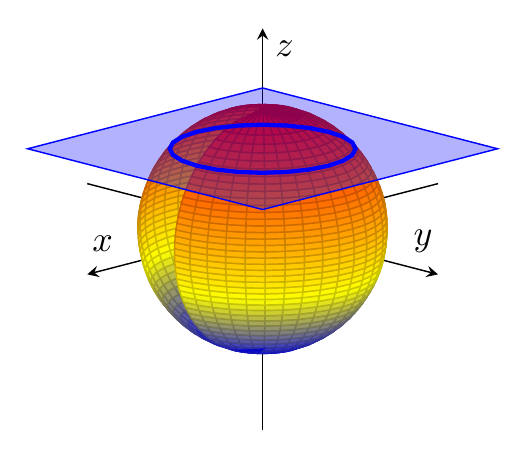
\begin{tikzpicture}[scale=1.3]
\begin{axis}[
    view={135}{15},
    axis equal,
    axis lines=middle,
    xlabel={$x$},ylabel={$y$},zlabel={$z$},
    grid=none,
    ticks=none,
    xmin=-5, xmax=5,
    ymin=-5, ymax=5,
    zmin=-5, zmax=5,
]
\addplot3[
    surf,
    samples=40,
    samples y=40,
    domain=-1:1,
    y domain=0:2*pi,
] (
    {3 * sqrt(1-x^2) * cos(deg(y))},
    {3 * sqrt(1-x^2) * sin(deg(y))},
    {3 * x}
);

\addplot3[
    surf,
    shader=flat,
    draw=Blue,
    fill=Blue,
    fill opacity=0.3,
    samples=2,
    domain=-4:4,
    y domain=-4:4,
] (
    {x},
    {y},
    {2}
);

\addplot3[
    domain=0:2*pi,
    Blue,
    very thick,
] (
    {sqrt(5)*cos(deg(x))},
    {sqrt(5)*sin(deg(x))},
    {2}
);
\end{axis}
\end{tikzpicture}
\end{figure}

Continuing with this idea, we can try to construct the general
shape of a surface by finding the traces. Let's take a look at
an example from our previous example.

\begin{minipage}{0.48\textwidth}
\begin{figure}[H]
\centering
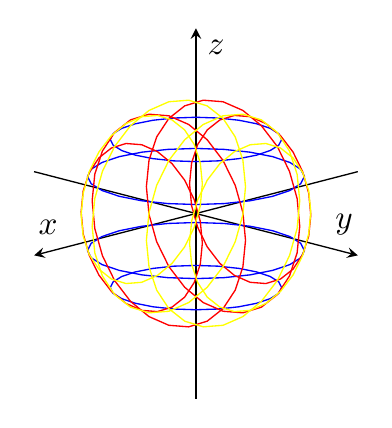
\begin{tikzpicture}[scale=1.2]
\begin{axis}[
    view={135}{15},
    axis equal,
    axis lines=middle,
    xlabel={$x$},ylabel={$y$},zlabel={$z$},
    grid=none,
    ticks=none,
    xmin=-5, xmax=5,
    ymin=-5, ymax=5,
    zmin=-5, zmax=5,
]
\foreach \z/\i in {
    -3/0,
    -2/5,
    -1/8,
     1/8,
     2/5,
     3/0
} {
    \addplot3[
        Blue,
        domain=0:2*pi,
    ] (
        {sqrt(\i)*cos(deg(x))},
        {sqrt(\i)*sin(deg(x))},
        {\z}
    );
}

\foreach \z/\i in {
    -3/0,
    -2/5,
    -1/8,
     1/8,
     2/5,
     3/0
} {
    \addplot3[
        Red,
        domain=0:2*pi,
    ] (
        {\z},
        {sqrt(\i)*cos(deg(x))},
        {sqrt(\i)*sin(deg(x))}
    );
}

\foreach \z/\i in {
    -3/0,
    -2/5,
    -1/8,
     1/8,
     2/5,
     3/0
} {
    \addplot3[
        Yellow,
        domain=0:2*pi,
    ] (
        {sqrt(\i)*cos(deg(x))},
        {\z},
        {sqrt(\i)*sin(deg(x))}
    );
}
\end{axis}
\end{tikzpicture}
\end{figure}
\end{minipage}
\hfill
\begin{minipage}{0.48\textwidth}
For surface $S$ defined as $x^2 + y^2 + z^2 = 9$, we can find the
trace of $S$ in $x = k$, $y = k$, and $z = k$. For each case,
we can see that there is no intersection for $|k| > 3$. Therefore
considering the equations for $|k| \leq 3$, we obtain the following
general structure. This indeed looks like a sphere!
\end{minipage}

Continuing, here is another example.

\begin{problem}{}{}
Find the general shape of the surface $\frac{x^2}{36} - \frac{y^2}{9}
+ \frac{z^2}{4} = 1$.
\end{problem}
\begin{solution}
To find the general shape of the surface, we can try to find different
traces in different planes to later combine them for a general shape.

\begin{minipage}{0.55\textwidth}
First, let's take a look at the traces in the plane $x = k$.
Substituting, we obtain an equation representing hyperbolas.
\[
\frac{z^2}{4} - \frac{y^2}{9} = 1 - \frac{k^2}{36}
\]
\end{minipage}
\hfill
\begin{minipage}{0.4\textwidth}
\begin{figure}[H]
\centering
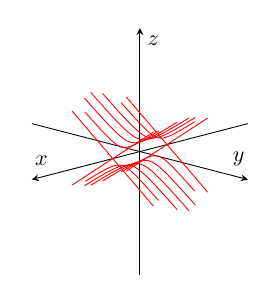
\begin{tikzpicture}[scale=0.8]
\begin{axis}[
    view={135}{15},
    axis equal,
    axis lines=middle,
    xlabel={$x$},ylabel={$y$},zlabel={$z$},
    grid=none,
    ticks=none,
    xmin=-20, xmax=20,
    ymin=-20, ymax=20,
    zmin=-20, zmax=20
]
\foreach \var in {-4,-2,0,2,4} {
    \addplot3[
        Red,
        domain=-2:2,
        samples=30,
        samples y=0,
        variable=\t
    ] (
        {\var},
        {3 * sqrt(1 - (\var)^2/36) * sinh(\t)},
        {2 * sqrt(1 - (\var)^2/36) * cosh(\t)}
    );

    \addplot3[
        Red,
        domain=-2:2,
        samples=30,
        samples y=0,
        variable=\t
    ] (
        {\var},
        {3 * sqrt(1 - (\var)^2/36) * sinh(\t)},
        {-2 * sqrt(1 - (\var)^2/36) * cosh(\t)}
    );
}

\foreach \var in {-6,6} {
    \addplot3[
        Red,
        domain=-3:3,
        samples=30,
        samples y=0,
        variable=\t
    ] (
        {\var},
        {3*\t},
        {2*\t}
    );

    \addplot3[
        Red,
        domain=-3:3,
        samples=30,
        samples y=0,
        variable=\t
    ] (
        {\var},
        {3*\t},
        {-2*\t}
    );
}
\end{axis}
\end{tikzpicture}
\end{figure}
\end{minipage}

Continuing, let's take a look at traces in the plane $y = k$.

\begin{minipage}{0.55\textwidth}
Substituting, we obtain $\frac{x^2}{36} + \frac{z^2}{4} =
1 + \frac{k^2}{9}$. Rearranging the equation, the following equation
of ellipse is obtained.
\[
\frac{x^2}{36 \left( 1 + \frac{k^2}{9} \right)}
    + \frac{z^2}{4 \left( 1 + \frac{k^2}{9} \right)}
= 1
\]
\end{minipage}
\hfill
\begin{minipage}{0.4\textwidth}
\begin{figure}[H]
\centering
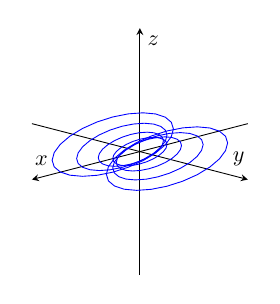
\begin{tikzpicture}[scale=0.8]
\begin{axis}[
    view={135}{15},
    axis equal,
    axis lines=middle,
    xlabel={$x$},ylabel={$y$},zlabel={$z$},
    grid=none,
    ticks=none,
    xmin=-20, xmax=20,
    ymin=-20, ymax=20,
    zmin=-20, zmax=20
]
\foreach \var in {-6,-4,-2,0,2,4,6} {
    \addplot3[
        Blue,
        domain=0:2*pi,
        samples y=0,
        variable=\t
    ] (
        {6 * sqrt(1 + (\var)^2/9) * cos(deg(\t))},
        {\var},
        {2 * sqrt(1 + (\var)^2/9) * sin(deg(\t))}
    );
}
\end{axis}
\end{tikzpicture}
\end{figure}
\end{minipage}

\begin{minipage}{0.55\textwidth}
Finally for $z = k$, we obtain the following equations
just like the case for $x = k$.
\[
\frac{x^2}{36} - \frac{y^2}{9} = 1 - \frac{k^2}{4}
\]
\end{minipage}
\hfill
\begin{minipage}{0.4\textwidth}
\begin{figure}[H]
\centering
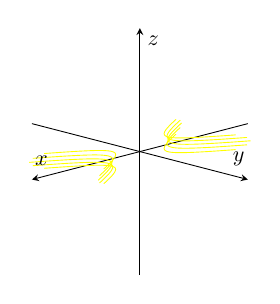
\begin{tikzpicture}[scale=0.8]
\begin{axis}[
    view={135}{15},
    axis equal,
    axis lines=middle,
    xlabel={$x$},ylabel={$y$},zlabel={$z$},
    grid=none,
    ticks=none,
    xmin=-20, xmax=20,
    ymin=-20, ymax=20,
    zmin=-3, zmax=3
]
\foreach \var in {-1,-0.5,0,0.5,1} {
    \addplot3[
        Yellow,
        domain=-1.5:1.5,
        samples=30,
        samples y=0,
        variable=\t
    ] (
        {6 * sqrt(1 - (\var)^2/4) * cosh(\t)},
        {3 * sqrt(1 - (\var)^2/4) * sinh(\t)},
        {\var}
    );

    \addplot3[
        Yellow,
        domain=-1.5:1.5,
        samples=30,
        samples y=0,
        variable=\t
    ] (
        {-6 * sqrt(1 - (\var)^2/4) * cosh(\t)},
        {3 * sqrt(1 - (\var)^2/4) * sinh(\t)},
        {\var}
    );
}
\end{axis}
\end{tikzpicture}
\end{figure}
\end{minipage}

Combining the traces, we obtain the general shape of the surface.

\begin{minipage}{0.46\textwidth}
\begin{figure}[H]
\centering
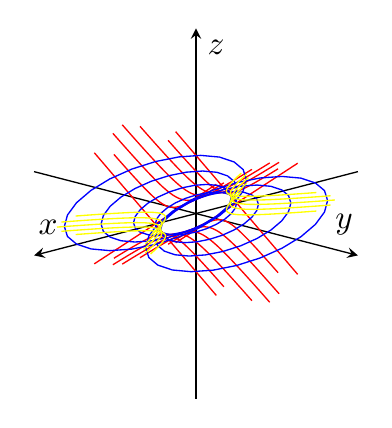
\begin{tikzpicture}[scale=1.2]
\begin{axis}[
    view={135}{15},
    axis equal,
    axis lines=middle,
    xlabel={$x$},ylabel={$y$},zlabel={$z$},
    grid=none,
    ticks=none,
    xmin=-20, xmax=20,
    ymin=-20, ymax=20,
    zmin=-20, zmax=20
]
\foreach \var in {-4,-2,0,2,4} {
    \addplot3[
        Red,
        domain=-2:2,
        samples=30,
        samples y=0,
        variable=\t
    ] (
        {\var},
        {3 * sqrt(1 - (\var)^2/36) * sinh(\t)},
        {2 * sqrt(1 - (\var)^2/36) * cosh(\t)}
    );

    \addplot3[
        Red,
        domain=-2:2,
        samples=30,
        samples y=0,
        variable=\t
    ] (
        {\var},
        {3 * sqrt(1 - (\var)^2/36) * sinh(\t)},
        {-2 * sqrt(1 - (\var)^2/36) * cosh(\t)}
    );
}

\foreach \var in {-6,6} {
    \addplot3[
        Red,
        domain=-3:3,
        samples=30,
        samples y=0,
        variable=\t
    ] (
        {\var},
        {3*\t},
        {2*\t}
    );

    \addplot3[
        Red,
        domain=-3:3,
        samples=30,
        samples y=0,
        variable=\t
    ] (
        {\var},
        {3*\t},
        {-2*\t}
    );
}

\foreach \var in {-6,-4,-2,0,2,4,6} {
    \addplot3[
        Blue,
        domain=0:2*pi,
        samples y=0,
        variable=\t
    ] (
        {6 * sqrt(1 + (\var)^2/9) * cos(deg(\t))},
        {\var},
        {2 * sqrt(1 + (\var)^2/9) * sin(deg(\t))}
    );
}

\foreach \var in {-1,-0.5,0,0.5,1} {
    \addplot3[
        Yellow,
        domain=-1.5:1.5,
        samples=30,
        samples y=0,
        variable=\t
    ] (
        {6 * sqrt(1 - (\var)^2/4) * cosh(\t)},
        {3 * sqrt(1 - (\var)^2/4) * sinh(\t)},
        {\var}
    );

    \addplot3[
        Yellow,
        domain=-1.5:1.5,
        samples=30,
        samples y=0,
        variable=\t
    ] (
        {-6 * sqrt(1 - (\var)^2/4) * cosh(\t)},
        {3 * sqrt(1 - (\var)^2/4) * sinh(\t)},
        {\var}
    );
}
\end{axis}
\end{tikzpicture}
\end{figure}
\end{minipage}
\hfill
\begin{minipage}{0.46\textwidth}
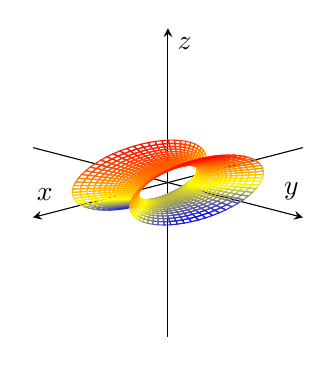
\begin{tikzpicture}
\begin{axis}[
    view={135}{15},
    axis equal,
    axis lines=middle,
    xlabel={$x$},ylabel={$y$},zlabel={$z$},
    grid=none,
    ticks=none,
    xmin=-20, xmax=20,
    ymin=-20, ymax=20,
    zmin=-20, zmax=20
]
\addplot3[
    mesh,z buffer=sort,
    samples=30,
    samples y=60,
    domain=-1.3:1.3,
    y domain=0:360,
    variable=\u,
    variable y=\v,
] (
    {6*cosh(\u)*cos(\v)},
    {3*sinh(\u)},
    {2*cosh(\u)*sin(\v)}
);
\end{axis}
\end{tikzpicture}
\end{minipage}
\end{solution}

Such surfaces are known as \textbf{hyperboloid}. Continuing with
surfaces, let's discuss quadratic surfaces.

Note that in coordinate plane, we call equations of the form
\[
Ax^2 + bxy + Cy^2 + Dx + Ey + F = 0
\]
a conic section. Some examples include parabola, hyperbola, circle,
and ellipse. Now, we could also generalize such equations in 3-space.

\begin{definition}{}{}
A \textbf{quadric surface} is known as the graph whose equation is
of the following form.
\vspace{-0.8\baselineskip}
\[
Ax^2 + By^2 + Cz^2 + Dxy + Eyz + Fzx + Gx + Hy + Iz + J = 0
\]
\end{definition}

For instance, the graph from our previous example is a quadric
surface.

To investigate in some quadric surfaces, let's take a look at
few examples. First, consider the examples of the following form.
\[
z^2 = \frac{x^2}{a^2} + \frac{y^2}{b^2}
\]
Considering the traces in planes $z = k$, we can notice that the
equation becomes
\[
\frac{x^2}{a^2 k^2} + \frac{y^2}{b^2 k^2} = 1
\]
which are ellipses or $(0, 0)$ if $k = 0$.

Similarly for $x = k$, we obtain
\[
\frac{z^2}{\left( \frac{k}{a} \right)^2}
    - \frac{y^2}{\left( \frac{bk}{a} \right)^2}
= 1
\]
which are hyperbolas. Continuing for $y = k$, we obtain the following
equation for hyperbolas.
\[
\frac{z^2}{\left( \frac{k}{b} \right)^2}
    - \frac{x^2}{\left( \frac{ak}{b} \right)^2}
= 1
\]
With the found traces, we could try finding the general shape of
the surface by combining them.

\begin{minipage}{0.48\textwidth}
\begin{figure}[H]
\centering
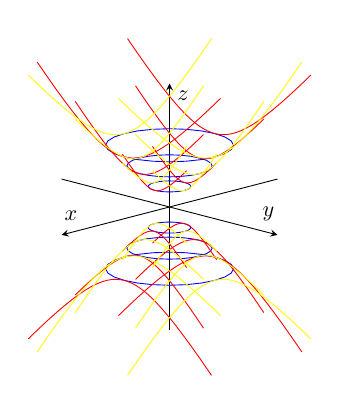
\begin{tikzpicture}[scale=0.8]
\begin{axis}[
    view={135}{15},
    axis equal,
    axis lines=middle,
    xlabel={$x$},ylabel={$y$},zlabel={$z$},
    grid=none,
    ticks=none,
    xmin=-12, xmax=12,
    ymin=-12, ymax=12,
    zmin=-12, zmax=12
]
\foreach \var in {-6,-4,-2,0,2,4,6} {
    \addplot3[
        Blue,
        domain=0:2*pi,
        samples y=0,
        variable=\t
    ] (
        {sqrt((\var)^2) * cos(deg(\t))},
        {sqrt((\var)^2) * sin(deg(\t))},
        {\var}
    );
}

\foreach \var in {-6,-4,-2,0,2,4,6} {
    \addplot3[
        Red,
        domain=-1.5:1.5,
        samples=30,
        samples y=0,
        variable=\t
    ] (
        {\var},
        {\var*sinh(\t)},
        {\var*cosh(\t)}
    );

    \addplot3[
        Red,
        domain=-1.5:1.5,
        samples=30,
        samples y=0,
        variable=\t
    ] (
        {\var},
        {\var*sinh(\t)},
        {-\var*cosh(\t)}
    );
}

\foreach \var in {-6,-4,-2,0,2,4,6} {
    \addplot3[
        Yellow,
        domain=-1.5:1.5,
        samples=30,
        samples y=0,
        variable=\t
    ] (
        {\var*sinh(\t)},
        {\var},
        {\var*cosh(\t)}
    );

    \addplot3[
        Yellow,
        domain=-1.5:1.5,
        samples=30,
        samples y=0,
        variable=\t
    ] (
        {\var*sinh(\t)},
        {\var},
        {-\var*cosh(\t)}
    );
}
\end{axis}
\end{tikzpicture}
\end{figure}
\end{minipage}
\hfill
\begin{minipage}{0.48\textwidth}
\begin{figure}[H]
\centering
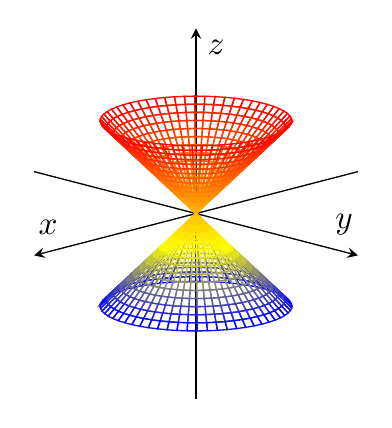
\begin{tikzpicture}[scale=1.2]
\begin{axis}[
    view={135}{15},
    axis equal,
    axis lines=middle,
    xlabel={$x$},ylabel={$y$},zlabel={$z$},
    grid=none,
    ticks=none,
    xmin=-20, xmax=20,
    ymin=-20, ymax=20,
    zmin=-20, zmax=20
]
\addplot3[
    mesh,z buffer=sort,
    samples=30,
    samples y=60,
    domain=-10:10,
    y domain=0:360,
    variable=\u,
    variable y=\v,
] (
    {\u*cos(\v)},
    {\u*sin(\v)},
    {\u}
);
\end{axis}
\end{tikzpicture}
\end{figure}
\end{minipage}

Such graphs are known as \textbf{elliptic cone}. Continuing,
let's try and graph surfaces of the following form with $a, b > 0$.
\[
y = \frac{x^2}{a^2} + \frac{z^2}{b^2}
\]
First, consider the trace in $y = k$. Note that if $k < 0$,
then there are no points since right-hand side is sum of squares.
Moreover rearranging the equations, we obtain the following equation
for ellipses.
\[
\frac{x^2}{ka^2} + \frac{z^2}{kb^2} = 1
\]
Continuing, we can consider traces in $x = k$ and $z = k$.
For each case, we can easily notice that it is the locus of quadratic
functions of $y$ with respect to $x$ and $z$. Graphing, we obtain
the general sketch.

\begin{minipage}{0.48\textwidth}
\begin{figure}[H]
\centering
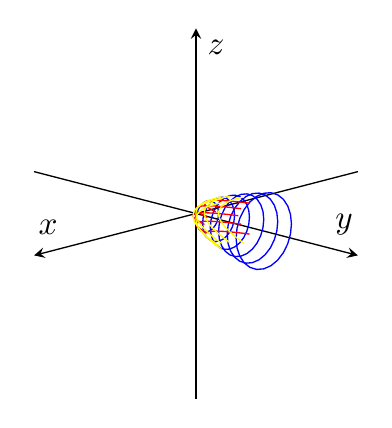
\begin{tikzpicture}[scale=1.2]
\begin{axis}[
    view={135}{15},
    axis equal,
    axis lines=middle,
    xlabel={$x$},ylabel={$y$},zlabel={$z$},
    grid=none,
    ticks=none,
    xmin=-12, xmax=12,
    ymin=-12, ymax=12,
    zmin=-12, zmax=12
]
\foreach \var in {0,1,2,3,4,5,6} {
    \addplot3[
        Blue,
        domain=0:2*pi,
        samples y=0,
        variable=\t
    ] (
        {sqrt(\var) * cos(deg(\t))},
        {\var},
        {sqrt(\var) * sin(deg(\t))}
    );
}

\foreach \var in {-1,-0.5,0,0.5,1} {
    \addplot3[
        Red,
        domain=-1.5:1.5,
        samples=30,
        samples y=0,
        variable=\t
    ] (
        {\t},
        {\t^2 + (\var)^2},
        {\var}
    );
}

\foreach \var in {-1,-0.5,0,0.5,1} {
    \addplot3[
        Yellow,
        domain=-1.5:1.5,
        samples=30,
        samples y=0,
        variable=\t
    ] (
        {\var},
        {(\var)^2 + \t^2},
        {\t}
    );
}
\end{axis}
\end{tikzpicture}
\end{figure}
\end{minipage}
\hfill
\begin{minipage}{0.48\textwidth}
\begin{figure}[H]
\centering
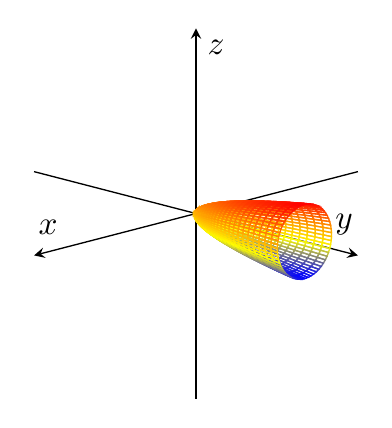
\begin{tikzpicture}[scale=1.2]
\begin{axis}[
    view={135}{15},
    axis equal,
    axis lines=middle,
    xlabel={$x$},ylabel={$y$},zlabel={$z$},
    grid=none,
    ticks=none,
    xmin=-20, xmax=20,
    ymin=-20, ymax=20,
    zmin=-20, zmax=20
]
\addplot3[
    mesh,z buffer=sort,
    samples=30,
    samples y=60,
    domain=0:4,
    y domain=0:360,
    variable=\u,
    variable y=\v,
] (
    {\u*cos(\v)},
    {\u^2},
    {\u*sin(\v)}
);
\end{axis}
\end{tikzpicture}
\end{figure}
\end{minipage}

This is known as \textbf{elliptic paraboloid}. There are much more
surfaces to discuss. For instance, \textbf{hyperboloid of two sheets}
are represented by $\frac{z^2}{c^2} - \frac{x^2}{a^2} -
\frac{y^2}{b^2} = 1$ while \textbf{hyperbolic paraboloid} is described
by $\frac{z}{c} = \frac{x^2}{a^2} - \frac{y^2}{b^2}$. Moreover,
\textbf{ellipsoid} are represented by $\frac{x^2}{a^2} +
\frac{y^2}{b^2} + \frac{z^2}{c^2} = 1$. For all such surfaces,
the following fact holds.

\begin{important}
Given a surface $S$ with equation $E(x, y, z)$, the equation of the
surface $S'$, obtained by translating $S$ by $a, b, c$ units in the
$x$, $y$, and $z$-direction respectively, is $E(x - a, y - b, z - c)$.
\end{important}

This is pretty straightforward with the same intuition we use for
2-space. This is it for this section! With different surfaces in
mind, let's discuss different ways to represent coordinates in
3-space.

\end{document}


